%%%%%%%%%%%%%%%%%%%%%%%%%%%%%%%%%%%%%%%%%%%%%%%%%%%%%%%%%%%%%%%%%%%%%%%%
\chapter{Fundamentals}
\label{sec:fundamentals}
%%%%%%%%%%%%%%%%%%%%%%%%%%%%%%%%%%%%%%%%%%%%%%%%%%%%%%%%%%%%%%%%%%%%%%%%

%=======================================================================
\section{Medical basics}
%=======================================================================

This section will give a basic overview about \gls{RSI} starting with a small introduction about the anatomy of the wrist.
The most important kinds of \gls{RSI} will be covered in more detail as well as how to diagnose these conditions and how to treat them.
Effectiveness of these treatments will be discussed too.
Since \gls{RSI} is a rather broad topic this section, as well as the whole thesis, will only cover \gls{RSI} of the wrist.

\subsection{Anatomy of the wrist}

\subsection{Endoscopic procedures}

In general, an endoscopic operation requires the surgeon to make a small incision at the surgical site and insert specialized surgical equipment into the incision.
During the operation the surgeon

\gls{RSI} symptoms

\gls{RSI} treatment

\subsection{Peretendonitis or tenosynovitis}

\subsection{Guyons canal syndrome}

\subsection{Carpal tunnel syndrome}

\gls{CTS} is not only the most common form of \gls{RSI} but in general the most prevalent neural injury\cite{ballestero2017effectiveness}.
In simplified terms \gls{CTS} is a disorder of the median nerve.
In the general population between 1\% and 4\% suffer from \gls{CTS}\cite{bongers2007carpal}.
15\% to 20\% of workers with a high risk for \gls{RSI} are reported to suffer from \gls{CTS}.
This high risk stems from workflows which require highly repetitive motions of the fingers and/or wrists like, for example, typing on a keyboard.
There is no total conses in the scientific literature on the definition of \gls{CTS}\cite{descatha2011comparison}.
In terms of physical symptoms some kind of tingling, pain, burning or general paraesthesia in the hands, fingers or wrists must be present for a prolonged period of time, even while sleeping.
Diminished grip strength might also be present.
Aside from physical symptoms, physical examination testing must also be conducted to properly diagnose \gls{CTS}.
An example ot these test would be the Phalen´s maneuver in which the test subject is instructed to place both hands together for a prolonged period of time as to fully flex both wrists.
The test indicates a case of \gls{CTS} if the subjects reports symptoms of paraesthesia, burning and/or numbness in the \gls{MND}.
\gls{MND} includes the wrist, palm and the first three digits.

Treatments for \gls{CTS} can be classified into two distinct groups:
\begin{itemize}
	\item Invasive treatments
	\item Non-invasive treatments
\end{itemize}
Invasive treatments encompass a multitude of surgical intervention.
A surgical intervention is normally only reserved for severe cases of \gls{CTS} or if all non-invasive treatments have failed\cite{scholten2007surgical}.
The goal of all surgical procedures is to reduce pressure on the median nerve.
This can be achieved by cutting the transverse carpal ligament(figure \ref{fig:carpal-tunnel-syndrome}), which subsequently increases wrist canal volume.
\begin{figure}
	\centering
	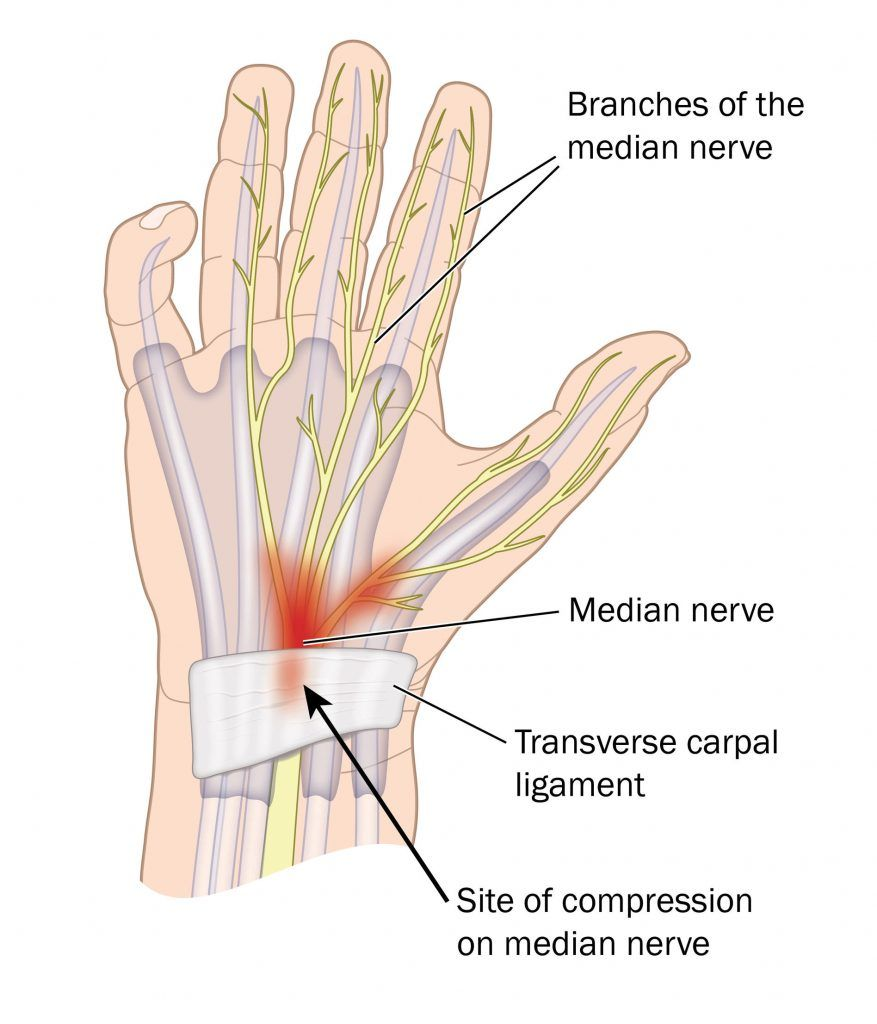
\includegraphics[width=0.6\linewidth]{figures/carpal-tunnel-syndrome}
	\caption{carpal tunnel syndrome (https://mylivinglocal.com/blog/carpal-tunnel-syndrome/)}
	\label{fig:carpal-tunnel-syndrome}
\end{figure}
A widely used procedure to achieve this effect is the standard \gls{OCTR}.
Over the years the standard \gls{OCTR} has been refined to only require a two to three centimeter long incision at the palm of the hand\cite{scholten2007surgical}.
No specialized tools are required for the operation.
In general, most patients report that \gls{CTS} related symptoms like daytime pain, tingling and numbness are reduced after \gls{OCTR}\cite{louie2013outcomes}.
The \gls{ECTR} is a less invasive form of the standard \gls{OCTR} procedure.
Since the the transverse carpal ligament can be cut from within the carpal tunnel overlaying tissue can be left intact.
This in turn should reduce post-operative morbidity\cite{scholten2007surgical}, although no data comparing post-operative morbidity between \gls{OCTR} and \gls{ECTR} is currently available.
In terms of patient satisfaction there seems to be no difference between the two surgical procedures\cite{atroshi2015extended}.
Medical complications after surgery are also relatively rare.
Structural damage to nerves, tendons or arteries only happens in 0.49\% of cases for \gls{OCTR} and 0.19\% for \gls{ECTR}\cite{benson2006complications}.
Even though the difference between \gls{OCTR} and \gls{ECTR} is statistically significant it can be said in general that both procedures are very safe to perform.
\textcolor{red}{ToDo: DOWNSIDES OF SURGICAL INTERVENTION}

Non-invasive treatments for \gls{CTS} consist of the following broadly defined groups:
\begin{itemize}
	\item Drug based treatments
	\item Movement restrictions
	\item Physical exercise
\end{itemize}

Drug based treatments include local corticosteriod injections, oral corticosteriods, \gls{NSAIDs} and Pyrodoxine.
Pyrodoxine is also better known as vitamine B\textsubscript{6}.
Most drug based treatments have the goal of providing short-term pain relief.
Multiple trials have confirmed corticosteriods, administered either orally or through injection, have short-term benefits\cite{van2007repetitive}.
The long-term effectiveness of corticosteriods, as well as other drugs, is unknown.
Most drugs used for \gls{CTS} treatment target the

Surgery
Injections
Stabilization

\gls{CTS} -> Treatment \cite{van2007repetitive}


%=======================================================================
\section{Game design basics}
%=======================================================================

This section will give an overview of the most important high level terms and theories in general game design.

Game loops

Winning states/Failure states

Randomness

How we learn to play. Game play literacy and other unknowns


%=======================================================================
\section{Graphics design basics}
%=======================================================================

Color theory

\subsection{Psychological impact of aesthetics}

ToDo: Describe what aesthetics are!

aesthetic scale in user tests to quantify aesthetics

Halo Effect

'prolongation of enjoyable experience' and 'increased motivation' is setting dependent \cite{sonderegger2010influence}

One of the most well known publications about impact of visual aesthetics in \gls{HCI} has been written by \fullcite{cawthon2007effect} <- NOT CORRECT REFERENCING.
In this publication the authors set up a study to compare the efficiency and effectiveness of different data visualization methods.
These methods where categorized through an online survey on a linear scale in terms of visual aesthetics, ranging from ugly to beautiful.
Even though the results where rather conclusive the study design itself needs to be criticized.
Visualization methods with beautiful aesthetics performed significantly better then ugly methods. 
But there was no indication if the different methods were even suited for handling the different study tasks.

Evaluation of visual design in state of the art

%=======================================================================
\section{Motivational theory}
%=======================================================================

Flow theory

%=======================================================================
\section{State of the art}
%=======================================================================

Flow theory

%-----------------------------------------------------------------------
\subsection{Unterkapitel}
%-----------------------------------------------------------------------

Bei der Verwendung von Gliederungsebenen gibt es Folgendes zu beachten:
\begin{itemize}
	\item Es sollten nicht mehr als 3 Gliederungstiefen nummeriert werden.
	\item Unterkapitel sind nur dann sinnvoll, wenn es auch mehrere Untergliederungen gibt. Ein Kapitel 2.1.1 sollte somit nur dann verwendet werden, wenn es auch 2.1.2 gibt.
	\item Oft ist es einfacher und besser verständlich, Aufzählungen als Text zu formulieren und somit weitere Gliederungsstufen zu vermeiden.
\end{itemize}

%-----------------------------------------------------------------------
\subsection{Abbildungen}
\label{sec:abbildungen}
%-----------------------------------------------------------------------

Beschreibungen zu Abbildungen und Tabellen stehen unter dem Bild. Jede Abbildung muss im Fließtext referenziert werden. In \LaTeX besitzen Abbildungen typischerweise Labels, welche zum referenzieren verwendet werden. Zudem plaziert \LaTeX die Abbildungen an geeigneten Stellen, was meistens auch wünschenswert ist. Falls das nicht gewünscht wird, kann es durch Optionen beeinflusst werden.

Abbildung \ref{fig:xxx} verdeutlicht  \dots\\
(siehe Abbildung \verb|\ref{<label>}|)

\begin{figure}
	\centering
	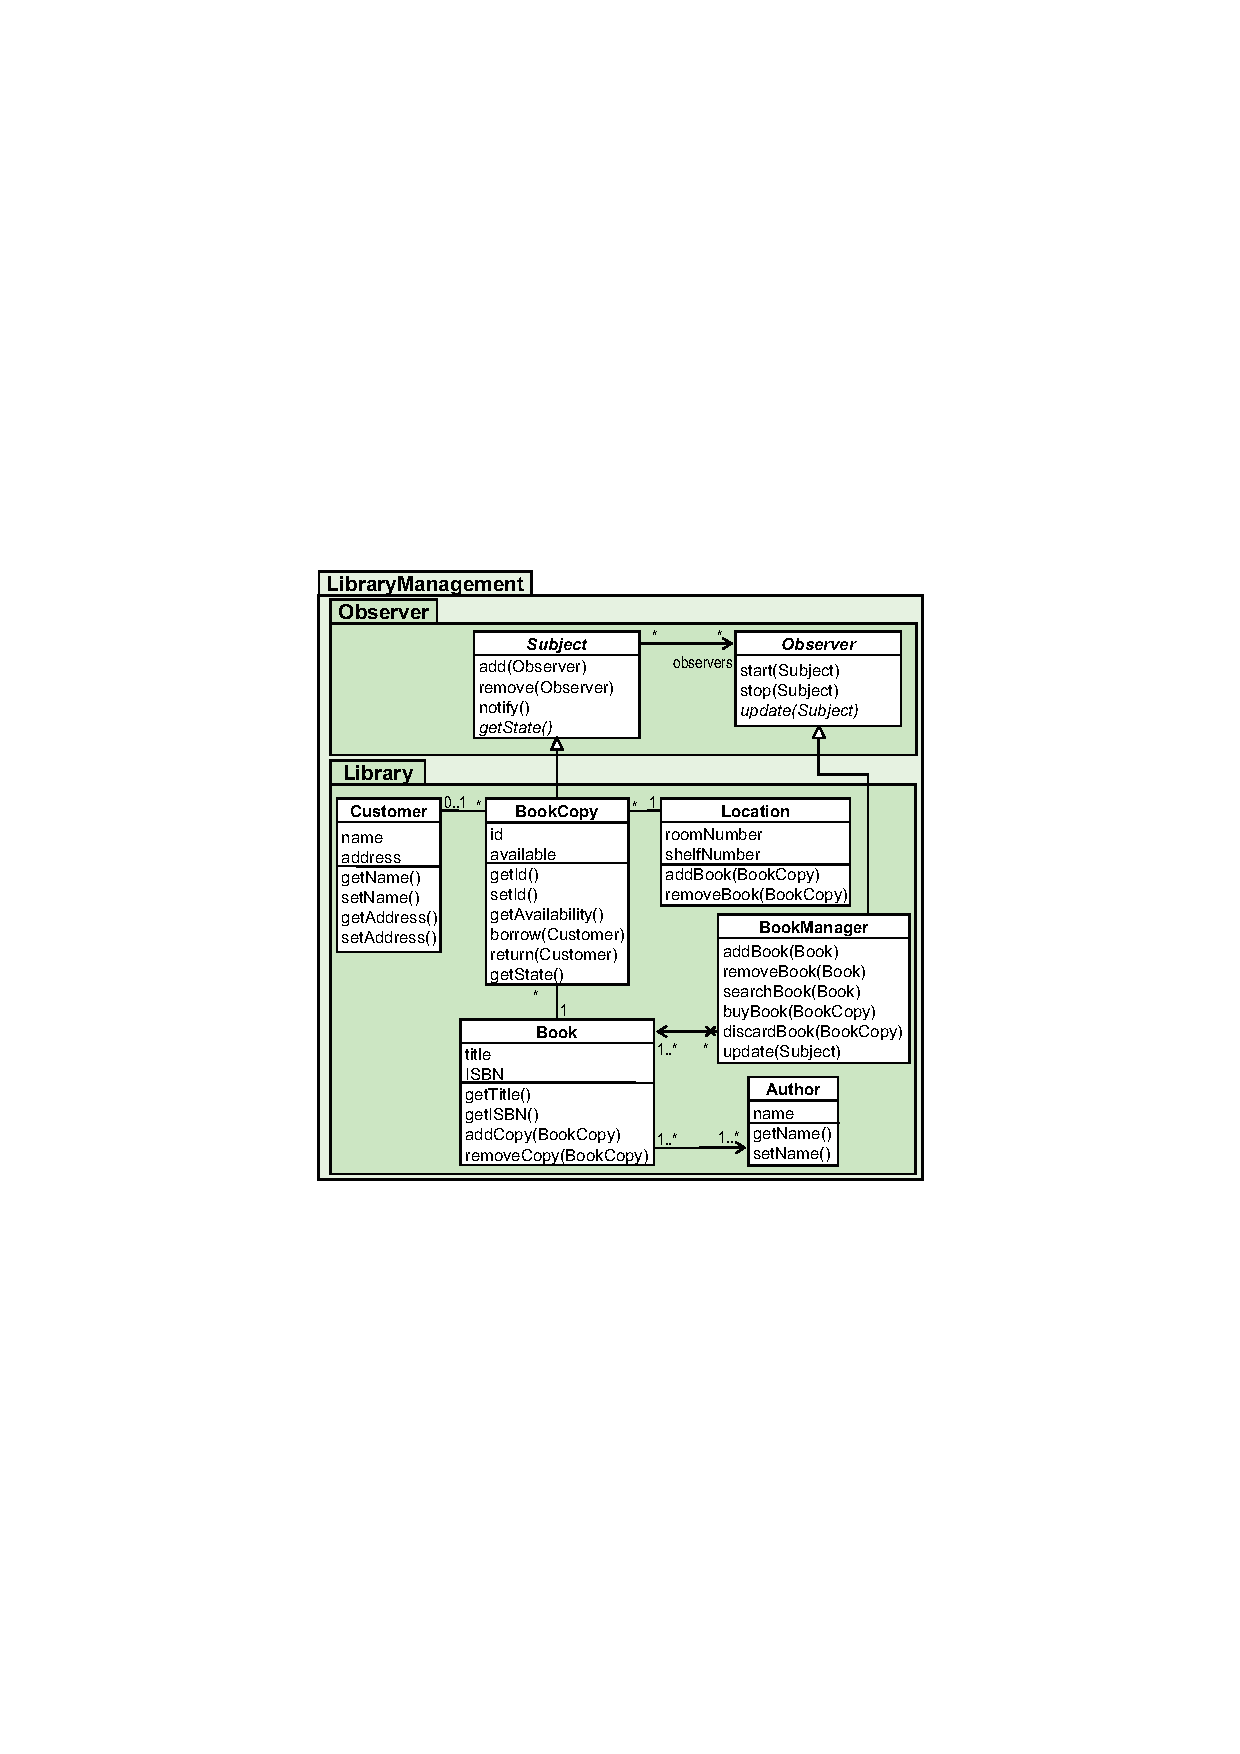
\includegraphics[width=0.4\linewidth]{figures/figure1}
	\caption{xxx (Quelle zitieren, wenn nicht selbst erstellt)}
	\label{fig:xxx}
\end{figure}

%-----------------------------------------------------------------------
\subsection{Tabellen}
%-----------------------------------------------------------------------

Jede Tabelle muss im Fließtext referenziertw werden. Für Tabellen gelten die selben Regeln, wie für Abbildungen (siehe dazu Abschnitt \ref{sec:abbildungen}).

Eine Beispiel einer Tabelle ist in Tabelle \ref{tab:xxx} zu finden:
\begin{table}
	\centering
	\begin{tabular}{| >{\bfseries}l | c | r | }
		\hline
			\rowcolor{orange} \bfseries Linksbündig & \bfseries Zentriert & \bfseries Rechtsbündig \\
		\hline
		\hline
			Zeile 1 & xxx & xxx \\\hline
			Zeile 2 & xxx & \dots \\\hline
			\multirow{2}{*}{Zeile3}
			& xxx & xxx \\\cline{2-3}
			& xxx & xxx \\\hline
		\hline
			\multicolumn{3}{| c |}{xxx} \\\hline
	\end{tabular}
	\caption{xxx (Quelle angeben)}
	\label{tab:xxx}
\end{table}

Bitte beachten Sie, dass Tabellen generell so einfach wie möglich gehalten werden sollen. Tabelle \ref{tab:xxx} dient unter anderem dazu Studierenden zu zeigen, wie Tabellen in \LaTeX\xspace erstellt werden können und wie Farben verwendet werden.